\section{Ermittlung der Anforderungen}
\subsection{Ermittlung der Stakeholder}
Bevor mit der Ermittlung der Anforderungen begonnen wird, müssen zuerst die Stakeholder identifiziert werden, die ein allgemeines Interesse an der zu entwicklenden Software, bzw. dem Tool haben. Dabei handelt es sich um Personen, die entweder von dem fertigen Produkt profitieren, oder die später das Produkt zu ihrer täglichen Arbeit einsetzen und daher ein Interesse am Funktionsumfang und der Benutzerfreundlichkeit haben. 

\subsubsection{Analyse der Stakeholder}
Im Falle des Business-Transformation-Trackers wurde folgende Stakeholder ermittelt:
\begin{itemize}
    \item[] \emph{Oberes Management:} Das obere Management des auftraggebenen Unternehmens ist der Auftraggeber für das Entwicklungsprojekt und hat daher besonderes Interesse in der erfolgreichen Fertigstellung des Projekts und der produktivsetzung der Software um somit Wertschöpfung zu generieren. Dazu kommt, dass das Ziel der Software die Unterstüzung der Mitarbeiter in den Projekten ist und sich durch den Einsatz eine Effizienzsteigerung und Qualitätsverbesserung erhofft wird. Dadurch besteht die Möglichkeit der Reputationssteigerung gegenüber potentiellen Kunden und somit einer gesteigerten Nachfrage im Vertrieb, was ebenfalls im besonderen Interesse des Managements liegt. In Persona tritt das obere Management im Entwicklungsprojekt als Bereichsleiter \glqq{}SAP Consulting and Development\grqq{} in Erscheinung.
    \item[] \emph{Mittleres Management:} Die Mitarbeiter des auftraggebenen Unternehmen im mittleren Management fungieren in der Regel in der Rolle eines Abteilungs- oder Projektleiters und haben daher ein besonderes Interesse an dem Funktionsumfang an der zu entwicklenen Software, da sie durch den Funktionsumfang direkt in den Projekten profitieren können. So profitieren sie beispielsweise von einer übersichtlichen Ansicht des gesamten Projekts und können durch Auswertungen besser das Projekt verwalten. Außerdem besitzen die Mitarbeiter des mittleren Managements ein Interesse darin, dass das Tool durch die Mitarbeiter verwendet wird, damit die darin geführten Daten stets auf dem aktuellen Stand sind. 
    \item[] \emph{Senior Consultants:} Senior Consultants sind erfahrene Mitarbeiter des auftraggebenen Unternehmens und arbeiten in der Regel als Projektleiter in kleineren Projekten oder als Teilprojektleiter in Projekten mit größerem Umfang. Sie haben ein großes Interesse im Funktionsumfang des BTT und sind auch sehr an der Übersichtlichkeit und Benutzerfreundlichkeit der grafischen Oberfläche interessiert, da sie, zusammen mit den Consultants, am intensivsten mit dem Programm arbeiten werden. Dabei stehen die Ziele der Datenkonsistenz und der generellen Verfügbarkeit des BTT im Vordergrund, damit eine reibungslose Arbeit ermöglicht wird.
    \item[] \emph{Consultants:} Die Consultants, bzw. Berater bilden den Kern der Mitarbeiterschaft des auftraggebenen Unternehmens und treten in der Regel als Projektmitarbeiter in Erscheinung. Sie bilden die größte Zielgruppe, da sie am häufigsten mit dem Programm arbeiten werden und dort den Großteil der Datenerfassung durchführen werden. Deshalb ist es vom besonderen Interesse, den Projektmitarbeitern die Arbeit mit dem Produkt möglichst einfach zu machen und besonders auf die Benutzerfreundlichkeit in der Entwicklung zu achten. Dazu kommt, das es wichtig ist, diese Stakeholdergruppe möglichst in die Entwicklung mit einzubeziehen, um Verbesserungsvorschläge und Ideen in die Anforderungen mit aufzunehmen. 
    \item[] \emph{Entwickler:} Die (SAP-)Entwickler des Auftraggebers spielen nur eine untergeordnete Rolle im Kontext des Business Transformation Tracker, da die Befüllung und Auswertung nicht in ihr Aufgabenfeld gehört. Denkbar sind dennoch Szenarien, in denen sie aufgefordert werden einzelne Einträge in dem Programm vorzunehmen, zu denen ihre Expertise benötigt wird. Auch besteht ein großes Interesse an Benutzerfreundlichkeit und Übersichtlichkeit, damit auch bei seltener Nutzung der Umgang mit dem Programm nicht schwer fällt.
    \item[] \emph{Kunden:} Weitere Stakeholder sind die Kunden des Auftraggebers, da diese ebenfalls Berührungspunkte mit dem Programm haben werden, wenn es Teil ihres Transformationsprojekts wird. Sie haben ein besonderes Interesse an der gesteigerten Effizienz und der gesteigerten Qualität ihrer Transformation, da dies für sie eingesparte Ressourcen in Form von weniger Projekttagen, weniger Aufwänden für die Transformation und geringere Wartungskosten im Anschluss durch die gesteigerte Qualität der Prozesse bedeutet. Dazu kommt, dass es dazu kommen kann, dass in größeren Projekten die Mitarbeiter des Kunden ebenfalls in direkten Kontakt mit dem BTT kommen, um bspw. bei der Erfassung der Prozesse zu unterstützen. Dadurch entsteht ein großes Interesse an der Übersichtlichkeit und der Benutzerfreundlichkeit, damit auch bei einmaliger Benutzung das gewünschte Resultat zustande kommt.
\end{itemize}

\subsubsection{Riskobewertung der Stakeholder}
Von den unterschiedlichen Stakeholdern gehen unterschiedliche Risiken im Bezug auf den Erfolg des Produkts aus. So gibt es auf der einen Seite ein unterschiedliches Konfliktpotential, das durch die unterschiedliche Mächtigkeit der Stakeholder, verschiedene Probleme im späteren Einsatz des Tools herbeiführen kann. So wäre es zum Beispiel denkbar, dass ein Consultant die Arbeit mit dem BTT verweigert, wenn seine persönlichen Anforderungen, in Form von Benutzerfreundlichkeit, außer Acht gelassen werden, oder, das ein Mitarbeiter des mittleren Managements, in Form eines Projektleiters, den Einsatz von Anfang an garnicht erst vorsieht, wenn er der Meinung ist, dass das Tool keinen Mehrwert bietet, wenn seine Anforderungen an das Programm, beispielsweise in Form von Verfügbarkeit und Zuverlässigkeit, nur unzulänglich erfüllt werden.
\begin{figure}[ht]
    \centering
    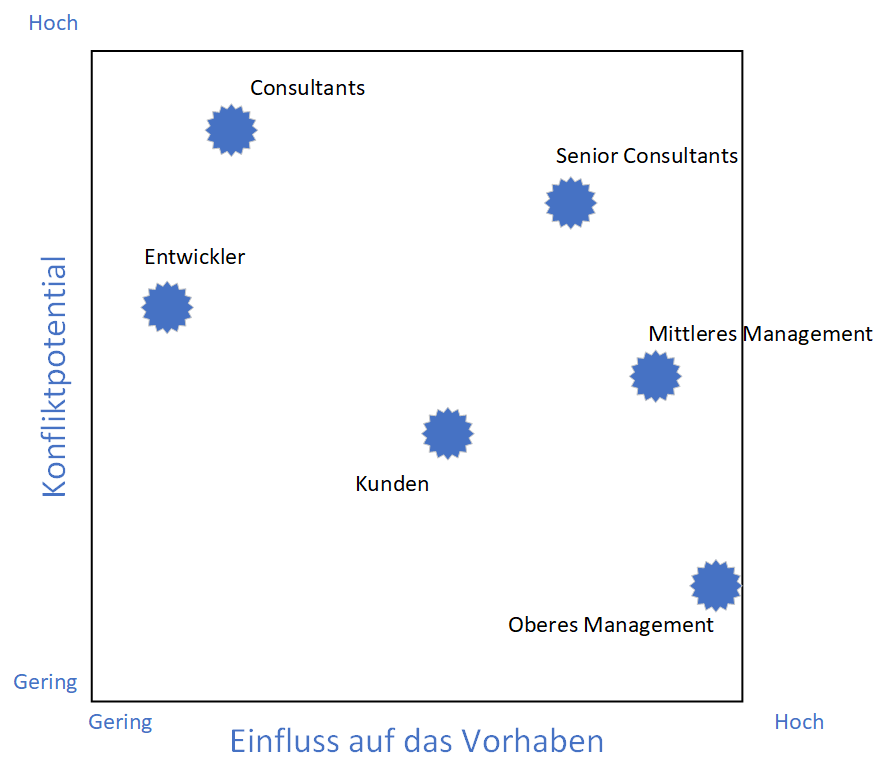
\includegraphics[scale=0.67]{Bilder/stakeholderRisiko.png}
    \caption[]{Subjektive Risikobewertung der genannten Stakeholder}
\end{figure}
Dieses Konfliktpotential lässt sich umgehen, indem die Personengruppen frühzeit in die Anforderungsermittlung mit eingebunden werden und sie dadurch, im Rahmen der Möglichkeiten, selbst bei der Produktentwicklung mitwirken können. Besonders bei Stakeholdern mit großer Macht und hohem Konfliktpotential ist es daher wichtig Maßnahmen zu definieren, wodurch dieses gesenkt werden kann.\footcite[Vgl.][S. 504 f.]{balzert}



\subsection{Erhebung der Anforderungen}
\subsubsection{Informationen durch den Auftraggeber}
Zur Ermittlung der Anforderungen fanden mehrere Gespräche mit dem Auftraggeber statt, in denen zum einen auf den aktuellen Ist-Zustand eingegangen wurde, aber auch Ideen und Umsetzungsvorschläge besprochen wurde. Diese Informationen wurden bereits in dem vorangegangenen Kapitel 5 in der Problemstellung und in der Beschreibung des Ist-Zustandes untergebracht und werden nun genutzt um daraus die Anforderungen an das in Auftrag gegebene Programm zu entwickeln. Während des Entwicklungsprozess besteht ein enger Kontakt zu dem Auftraggeber, wodurch auftretene Rückfragen schnell beantwortet werden können. 

\subsubsection{Befragung im Unternehmen}
Um von möglichst vielen Stakeholdern Anforderungen an eine Neuentwicklung des Business Transformation Trackers zu erhalten, wurde mit den Mitarbeitern des auftraggebenen Unternehmen, die bereits mit der aktuellen Umsetzung des BTT, bzw. seinem Vorgänger, gearbeitet haben, eine Onlinebefragung durchgeführt. Ziel der Befragung war es zum einen das generelle Meinungsbild der Mitarbeiter zu dem BTT zu erfassen und zum anderen mögliche Verbesserungsvorschläge und Ideen der Stakeholder aufzugreifen, um daraus Anfoderungen an einen Neuaufbau des BTT zu entwickeln. Die Umfrage richtet sich dabei an alle internen Stakeholder, das heißt an die Mitarbeiter des oberen und mittleren Mangements, an die Senior Consultants, Consultants und Entwickler. Dadurch soll ein möglichst breites Bild entstehen, dass alle Interessen abdeckt, sodass kein Stakeholder vernachlässigt wird.\\Die Umfrage wurde mit der Online-Plattform \glqq{}Microsoft Teams\grqq{} umgesetzt, das Bestandteil der im Unternehmen eingesetzen Softwaresuite \glqq{}Microsoft 365\grqq{} ist. Die Umfrage wurde anonym durchgeführt, mit der Möglichkeit am Ende freiwillig seine Kontaktdaten anzugeben, um Rückfragen zu den gegebenen Antworten und Vorschlägen zu ermöglichen. Der Fragenkatalog bestand aus drei Abschnitten, zuerst allgemeine Fragen zur Person und zur Position im Unternehmen, als nächstes mit Fragen zur Meinung über den BTT und zum Schluss mit der Möglichkeit Verbesserungsvorschläge und Ideen anzugeben. Um dem Betriebsklima im Unternehmen gerecht zu werden, wurde in der Umfrage auf die förmliche Anrede der Befragten verzichtet.

\subsubsection{Auswertung der Umfrage}

\subsection{Spezifikation der Anforderungen}
Im nun folgenden Unterkapitel werden die im letzten Kapitel, durch Onlinebefragung und in persönlichen Gesprächen, ermittelten Anforderungen spezifiziert, das heißt, systematisch ausgewertet. Es wird aufgrund einer nichtvorhandenen Ausschreibung des Projekts und des geringen Projektumfangs auf ein seperates Lasten- und Pflichtenheft verzichtet und stattdessen die Anforderungen in der hier beginnenden \glqq{}Requirements Specification\grqq{}, zu deutsch \glqq{}Anforderungsspezifikation\grqq{}, niedergeschrieben. Dazu wird sich an der von Helmut Balzert beschriebenen \glqq{}Schablone[n] für Lastenheft, Pflichtenheft und Glossar\grqq{}\footcite[S. 492]{balzert} orientiert. In dieser werden zuerst die Visionen und Ziele des Entwicklungsprojekt verfasst, danach die Rahmenbedingungen denen die Entwicklung unterliegt, im Anschluss der technische Kontext, in dem sich die Entwicklung abspielt und dann erst die funktionalen Anforderungen, die die Kernfunktionalität des Systems beschreiben gefolgt von den nichtfunktionalen Anforderungen, bzw. den Qualitätsanforderungen, in denen die messbare Qualität und das Verhalten des Systems beschrieben wird.\footcite[Vgl.][S. 492 ff.]{balzert}. Die Anforderungen sind natursprachlich verfasst und verfügen über einen einzigartigen Identifikator, um im späteren Verlauf auf sie verweisen zu können. Diese sind so aufgebaut, dass \glqq{} [j]ede Anforderung [..] mit einem Buchstaben [beginnt] [...], gefolgt von einer Zahl, eingschlossen in Schrägstriche. Der Anforderungstyp wird durch einen Buchstaben gekennzeichnet [...]. Am Anfang werden  die Zahlen in Zehnerschritten durchnummeriert, sodass spätere fachlich dazugehörige Anforderungen zwischgefügt werden können.\grqq{} \footcite[S. 493]{balzert}

\subsubsection{Visionen und Ziele}
Die hier aufgezählten Visionen und Ziele sind Ausdruck der mit dem fertigen Produkt zu erreichenden Zukunft. Visionen sind dabei abstrakter und generisch verfasst, Ziele konkretisieren diese dann im Anschluss.\footcite[Vgl.][S. 457]{balzert}
\begin{itemize}
    \item[] \emph{/V10/} Der Auftraggeber soll durch den Business Transformation Tracker eine Qualitätssteigerung und Effizienzverbesserung in seinen Transformationsprojekten erreichen.
    \item[] \emph{/V20/} Die Anwender sollen mit dem Business Transformation Tracker während des gesamten Projektzeitraums die in SAP umgesetzten Prozesse erfassen und nachverfolgen können.
    \item[] \emph{/V30/} In jedem adesso active transformation -Projekt soll der Business Transformation Tracker eingesetzt werden.
    \item[] \emph{/V40/} Das Produkt soll dem Anwender eine angenehme Userexperience bieten und muss ihn in seiner Arbeit produktiv unterstützen.
\end{itemize}

\begin{itemize} 
    \item[] \emph{/Z10/} Der Business Transformation Tracker soll zu jedem Zeitpunkt den aktuellen Fortschritssgrad ausgeben können, um schnell eine Übersicht zu erhalten.
    \item[] \emph{/Z20/} Dem Anwender soll es möglich sein, unterschiedliche Projekt aufrufen zu können.
    \item[] \emph{/Z30/} Die Ziele der Informationssicherheit (Authentizität, Vertraulichkeit, Integrität) dürfen nicht verletzt werden.
    \item[] \emph{/Z40/} Alle bereits jetzt implementierten Funktionen werden in die Neuentwicklung übernommen.         
    \item[] \emph{/Z50/} Der Business Transformationen Tracker soll den Funktionsumfang der jetzigen Lösung überbieten.  
    \item[] \emph{/Z60/} Das Anlegen eines Projektes im BTT dauert nicht länger als eine Minute.
    \item[] \emph{/Z70/} Die Erstellung eines Prozesschrittes ist dem Benutzer intuitiv möglich.
    \item[] \emph{/Z80/} Die Anwendung ist auf allen verbreiteten System einsetzbar.
    \item[] \emph{/Z90/} 
    \item[] \emph{/Z100/} 
\end{itemize}

\subsubsection{Rahmenbedingungen}

\begin{itemize}
    \item[] \emph{/R10/}
    \item[] \emph{/R20/}
\end{itemize}

\subsubsection{Kontext und Überblick}

\begin{itemize}
    \item[] \emph{/K10/}
    \item[] \emph{/K20/}
\end{itemize}

\subsubsection{Funktionale Anforderungen}

\begin{itemize}
    \item[] \emph{/F10/}
    \item[] \emph{/F20/}
\end{itemize}

\subsubsection{Qualitätsanforderungen}

\begin{itemize}
    \item[] \emph{/Q10/}
    \item[] \emph{/Q20/}
\end{itemize}
